\documentclass[11pt]{article}
\usepackage[utf8]{inputenc}
\usepackage[T1]{fontenc}
\usepackage{fixltx2e}
\usepackage{graphicx}
\usepackage{longtable}
\usepackage{float}
\usepackage{wrapfig}
\usepackage{rotating}
\usepackage[normalem]{ulem}
\usepackage{amsmath}
\usepackage{textcomp}
\usepackage{marvosym}
\usepackage{wasysym}
\usepackage{amssymb}
\usepackage{acl2015}
\usepackage{times}
\usepackage{url}
\usepackage{latexsym}
\usepackage{forest}
\usepackage[linesnumbered]{algorithm2e}
\DeclareMathOperator*{\argmin}{arg\,min}
\DeclareMathOperator*{\argmax}{arg\,max}
\newcommand{\BigO}[1]{\ensuremath{\operatorname{O}\bigl(#1\bigr)}}

\title{CKY Parsing With Independence Constraints}
\author{Joseph Irwin \\
  Graduate School of Information Science\hspace{1em} \\
  Nara Institute of Science and Technology\hspace{1em} \\
  {\tt joseph-i@is.naist.jp} \\\And
  Yuji Matsumoto \\
  Graduate School of Information Science \\
  Nara Institute of Science and Technology \\
  {\tt matsu@is.naist.jp} \\}

\begin{document}

\maketitle

\begin{abstract}
The CKY algorithm is an important component in many natural language
parsers. We propose a novel type of constraint for context-free
parsing called independence constraints. Based on the concept
of independence between words, we show how these constraints can be
used to reduce the work done in the CKY algorithm. We demonstrate a
classifier which can be used to identify boundaries between
independent words in a sentence using only surface features, and show
that it can be used to speed up a CKY parser. We investigate the
trade-off between speed and accuracy, and indicate directions for
improvement.
\end{abstract}

\section{Introduction}
\label{sec-1}



The CKY algorithm is an \BigO{|G|n^3} dynamic programming
algorithm for finding all of the possible derivations of a sentence in
a context-free language. Its complexity depends on both the sentence
length $n$ and the size of the grammar $|G|$. Methods for improving
parse accuracy typically increase the size of the grammar 
\cite{Klein2003,Petrov2007} or even the exponent of $n$ \cite{Eisner1999}. 
More powerful “deep” grammar formalisms multiply the computational
complexity even more \cite{Bangalore1999}.

A common technique for speeding up such parsers is coarse-to-fine
parsing, where input is first parsed using a much simpler (and thus
smaller) grammar, and the content of the chart is then used to
constrain the search over the final grammar
\cite{Torisawa2000,Charniak2005,Petrov2007}. Even with a much smaller
grammar, the CKY algorithm may be expensive---Roark et al. (2012)
report that the initial CKY step in the Berkeley Parser takes half of
the total parse time.

Other techniques can be used to prune cells in the chart. Roark et al.
(2012) use a finite-state model to label words that do/don't begin/end
spans, and skip cells that don't satisfy the labels. Bodenstab et al.
(2011) directly apply a classifier to each cell to decide how many
spans to keep. Both approaches reduce the work done by the parser
while preserving accuracy.

We propose a novel type of top-down constraint for a CFG parser that
we call independence constraints, described in Section 2. In Section 3
we show how the CKY algorithm can be easily modified to accommodate
these constraints, and in Section 4 we describe a classifier which can
provide the constraints to a parser. We integrate the constraints into
the Stanford Parser CKY implementation and show the results in Section 5.

\section{Independence Constraints}
\label{sec-2}

\begin{figure}
\centering
\begin{forest}
  [S
   [NP [DT [ $_0$ This $_1$]]]
   [VP
    [VB [is $_2$]]
    [NP [DT [an $_3$]]
        [NN [example $_4$]]]]
   [{.} [{.} $_5$]]
  ]
\end{forest}
\caption{In this tree `This' and `is' are independent, while `is' and `an' are not.}
\label{fig:independence}
\end{figure}

We propose a concept we call \textbf{independence}. Given a sentence $s = w_1
w_2 \dots w_n$ and a context-free derivation (parse tree) $t$ of $s$,
words $w_i$ and $w_{i+1}$ are \textbf{independent} if every node in $t$ that
dominates both $w_i$ and $w_{i+1}$ also dominates $w_1$ and $w_n$.
Furthermore, if $w_i$ and $w_{i+1}$ are independent, then $\forall
j,k$ s.t. $j \leq i$ and $k > i$, $w_j$ and $w_k$ are independent.
Less formally, if the children of the top node of a parse tree were
split into separate subtrees, two words are independent if they would
end up in different subtrees.

An example is shown in Figure \ref{fig:independence}. Here, `This' and
`is' are independent, as are `example' and `.'. The independent spans
are (`This'), (`is', `an', `example'), and (`.'), with boundaries 1
and 4. The independent spans and independent span boundaries can be
derived straightforwardly from the definition of independent words:
the locations between consecutive words which are independent are the
independent span boundaries, and the independent spans are simply the
spans in between consecutive boundaries.

\section{Modifying The CKY Algorithm With Independence Constraints}
\label{sec-3}

Conceptually, if a CKY parser knows the locations of the
independent span boundaries for a sentence, it can perform the normal
CKY algorithm for each independent span separately, and simply join
the spans at the top of the tree to finish the parse, thereby avoiding
work which would otherwise be done while still obtaining the desired
1-best parse. Two issues make the task more complicated than this.

The first complication is that if we assume that the independent boundaries
will be identified automatically, we must allow for errors. If a
location which is not an independent span boundary is given as one,
the parser will make an error it would not have otherwise. On the
other hand, if a location which is an independent span boundary is not
marked as such, the parser may account for this at the cost of not
achieving the minimum computation possible. By allowing for this
second type of error, the algorithm is made more robust, and allows
the independent boundary identification step to prioritize precision
over recall to lessen negative impact on the parser's accuracy.

The second issue is caused by the binarization of the context-free grammar used
in the CKY algorithm. Because the CKY algorithm requires a binary grammar, any
rules in the original grammar that have more than two symbols on the right-hand
side must be converted into a sequence of binary rules. The extra rules created
in this process are called incomplete\footnote{E.g., if a rule $A \rightarrow B C D$ becomes $@_{BC} \rightarrow B C$ and
$A \rightarrow @_{BC} D$, then the former is \emph{incomplete} and the latter is \emph{complete}.} rules. The topmost span in
particular will usually need to be constructed in several steps, applying
multiple incomplete rules before creating a complete span. If the grammar rules
are always binarized from the left (right), then only cells on the left (right)
edge of the chart can affect the top span; however, the grammar used in our
parser is binarized ``head-outward'' \cite{Klein2003}, which means that
potentially any cell in the chart can be used to create the top span.

The combination of these two issues means that in order to correctly parse a
sentence when an independent span boundary is missing from the input the
modified CKY algorithm must process incomplete rules even at positions in the
chart that cross a boundary. Thus in the modified algorithm, cells which do not
cross an independent boundary are processed normally, and in cells which do
cross a boundary the algorithm will avoid looping over complete binary rules.\footnote{While boundary-crossing cells depend on non-crossing
cells, the reverse is not the case; thus the non-crossing cells can
all be processed before the crossing cells, or the cells can be looped
over in the regular order, with a check inside the loop. While this may have
implications for e.g. parallelization, we do not explore this idea further here.}
Figure \ref{fig:chart} shows an example CKY chart where boundary-crossing cells are
colored gray.

\begin{figure}[t]
  \centering
  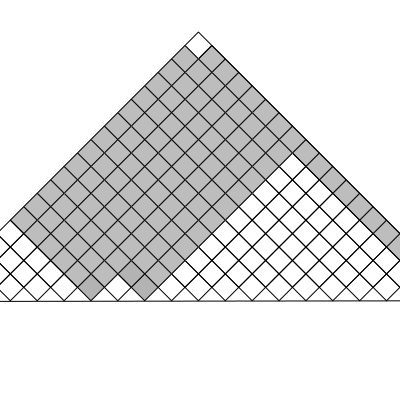
\includegraphics[width=6cm]{chart-constraints}
  \caption{Example of a CKY chart with independence constraints. In the gray cells the modified algorithm will only loop over incomplete rules. \label{fig:chart}}
\end{figure}

\subsection{How much work can we expect to save?}
\label{sec-3-1}
\label{sec:comp-saved}

\begin{algorithm}[t]
  \caption{The CKY algorithm. $T_{i,j}$ is the cell corresponding to words $w_i \dots w_{j-1}$.\label{alg:cky}}
  \DontPrintSemicolon
  \For {$1 \le i \le n$}{
    $T_{i,i+1} \gets \{A|A\rightarrow a \in G \wedge w_i = a\}$
  }
  \For {$2 \le j \le n$}{
    \For {$1 \le i \le n-j+1$}{
      \For {$i < k < i+j$}{
        $T_{i,i+j} \gets \{A|A\rightarrow BC \in G \wedge B \in T_{i,k} \wedge C \in T_{k,i+j} \}$\;
      }
    }
  }
\end{algorithm}

The core of the CKY algorithm is shown in Algorithm \ref{alg:cky}. For our
purposes, we can consider the amount of work done in the CKY algorithm to be the
number of binary edges visited in the inner loop (lines 4-10). For each cell the
algorithm iterates over the binary rules in the grammar, calculating the
probability of the left-hand-side at each split point. The number of these
binary edges is

\begin{equation}
|G|\left[\frac{n^3}{6} - \frac{n}{6}\right]
\end{equation}

The amount of work saved depends on the number and locations of the
independent span boundaries, as well as the proportion of
complete rules in the grammar, denoted $\frac{|G_{comp}|}{|G|}$. We
can consider two idealized scenarios: a) one boundary at $\frac{n}{K}$,
and b) $K-1$ boundaries at $\frac{n}{K}, \frac{2n}{K}, \dots,
\frac{(K-1)n}{K}$, where $K$ is an integer $1 < K < n$.

For the first case, the ratio of work saved approaches

\begin{equation}
\frac{|G_{comp}|}{|G|} \left[ \frac{3}{K} - \frac{3}{K^2} \right]
\end{equation}

as $n$ grows. This limit converges quickly for $n \ge 10$. If we
approximate $|G_{comp}|/|G|$ as 0.5 (for the grammar used by the parser in
Section \ref{sec:parser}, it is $\approx .54$), then for
$K=2,3,4,\dots$, the values are $\frac{3}{8}, \frac{1}{3}, \frac{3}{32}, \dots$
Intuitively, for one boundary, the best location
is exactly in the center of the sentence, and the upper limit on how
much work is saved is about 37\%.

For the case of $K-1$ boundaries equally spaced, the ratio is

\begin{equation}
\frac{|G_{comp}|}{|G|}\frac{K^2 - 1}{K^2}
\end{equation}

The values for $K=2,3,4,\dots$ are $\frac{3}{8}, \frac{4}{9}, \frac{15}{32}, \dots$
Clearly, the smaller pieces a sentence can be
divided into the less work the parser will do; however, realistically
most sentences will not have a large number of independent spans, and
they will not be equal in length. We might take $K=3$ as best-case
estimate, giving us about 44\%. Thus we can guess that a parser will be
able to save around 35-45\% of the work it does in the CKY algorithm
loop by using independence constraints.

The derivations of Equations 1-3 are shown in Appendix~\ref{sec:derivation-equations}.

\section{Classifying Independent Span Boundaries}
\label{sec-4}

In order to use independence constraints in a parser, we need to be
able to identify boundaries between independent words in a sentence
using only surface features (words and part-of-speech tags). We
created a binary classifier which, given a POS-tagged sentence and a
position between two words, decides whether those two words are
independent or not. Our classifier currently uses only POS tags as
features. We used \texttt{opal} \cite{Yoshinaga2010}, a tool for fast online
classification, to train and test the models, training on sentences
from Penn Treebank section 02-21 and testing on section 22. We set
opal to use the passive-aggressive perceptron update, and output
probabilities in order to use a threshold to trade off precision and
recall.

\subsection{Features}
\label{sec-4-1}

\begin{table*}[tbp]
%\resizebox{12cm}{!}{

\begin{tabular}{lrrrrrrrrrr}
Features & \#feats & Acc & Prec & Rec & F$_{\text{1}}$ & F$_{\text{0.5}}$ & TP & FP & FN & TN\\
\hline
p & 37001 & 93.71 & 80.73 & 70.49 & 75.27 & 78.45 & 3679 & 878 & 1540 & 32320\\
P$_{\text{0}}$ & 33167 & 87.16 & 51.69 & 83.98 & 63.99 & 55.99 & 4383 & 4097 & 836 & 29101\\
\hline
p,P$_{\text{0}}$ & 70168 & 95.21 & 87.38 & 75.65 & 81.09 & 84.75 & 3948 & 570 & 1271 & 32628\\
p,P$_{\text{1}}$ & 37055 & 94.81 & 78.38 & 85.38 & 81.73 & 79.69 & 4456 & 1229 & 763 & 31969\\
p,P$_{\text{2}}$ & 39336 & 95.34 & 84.25 & 80.76 & 82.47 & 83.53 & 4215 & 788 & 1004 & 32410\\
p,P$_{\text{3}}$ & 46861 & 95.04 & 89.47 & 71.95 & 79.76 & 85.31 & 3755 & 442 & 1464 & 32756\\
\hline
p,P$_{\text{0}}$,P$_{\text{1}}$ & 70222 & 95.48 & 88.95 & 76.16 & 82.06 & 86.06 & 3975 & 494 & 1244 & 32704\\
p,P$_{\text{0}}$,P$_{\text{2}}$ & 72503 & 95.09 & 88.28 & 73.60 & 80.27 & 84.89 & 3841 & 510 & 1378 & 32688\\
p,P$_{\text{0}}$,P$_{\text{3}}$ & 80028 & 94.84 & 88.81 & 70.99 & 78.91 & 84.56 & 3705 & 467 & 1514 & 32731\\
\hline
p,P$_{\text{1}}$,P$_{\text{2}}$ & 39390 & 95.27 & 80.99 & 85.21 & 83.04 & 81.80 & 4447 & 1044 & 772 & 32154\\
p,P$_{\text{1}}$,P$_{\text{3}}$ & 41553 & 95.44 & 89.05 & 75.74 & 81.86 & 86.03 & 3953 & 486 & 1266 & 32712\\
\hline
p,P$_{\text{0}}$,P$_{\text{1}}$,P$_{\text{2}}$,P$_{\text{3}}$ & 82417 & 95.35 & 86.89 & 77.49 & 81.92 & 84.83 & 4044 & 610 & 1175 & 32588\\
\end{tabular}

%}
\caption{Results of classifier using different combinations of features.}
\label{tbl:feature-evaluation}
\end{table*}

We use only part-of-speech tags to create features for the classifier
(adding lexical or other features is left to future work). The
property of independence between two words is inherently global, as it
can be affected by structure arbitrarily far away. Thus we have both
local and global features. The global features are furthermore
distinguished by \textbf{POS level}, explained in detail later. The specific
feature templates are shown below:

\subsubsection{Local Features}
\label{sec-4-1-1}
\begin{enumerate}
\item Left
\label{sec-4-1-1-1}
\begin{itemize}
\item $t_{k-1}$
\item $t_{k-2},t_{k-1}$
\item $t_{k-3},t_{k-2},t_{k-1}$
\end{itemize}

\item Right
\label{sec-4-1-1-2}
\begin{itemize}
\item $t_{k}$
\item $t_{k},t_{k+1}$
\item $t_{k},t_{k+1},t_{k+2}$
\end{itemize}
\end{enumerate}

\subsubsection{Global Features}
\label{sec-4-1-2}

Below, $t^{l}_{i}$ is the $i$ th POS tag in the $l$-level POS tag sequence.

\begin{enumerate}
\item Left
\label{sec-4-1-2-1}
\begin{itemize}
\item $t^l_{i}$ for $1 \le i < k - 1$, $l \in {0,1,2,3}$
\item $t^l_{i},t^l_{i+1}$ for $1 \le i < k - 2$, $l \in {0,1,2,3}$
\item $t^l_{i},t^l_{i+1},t^l_{i+2}$ for $1 \le i < k - 3$, $l \in {0,1,2,3}$
\end{itemize}

\item Right
\label{sec-4-1-2-2}
\begin{itemize}
\item $t^l_{i}$ for $k \le i < n - 1$, $l \in {0,1,2,3}$
\item $t^l_{i},t^l_{i+1}$ for $k \le i < n - 2$, $l \in {0,1,2,3}$
\item $t^l_{i},t^l_{i+1},t^l_{i+2}$ for $k \le i < n - 3$, $l \in {0,1,2,3}$
\end{itemize}
\end{enumerate}

\subsection{POS Level}
\label{sec-4-2}

\begin{table}[tbp]
\centering
\scriptsize

\begin{tabular}{llllllll}
Lvl0 & Lvl1 & Lvl2 & Lvl3 & Lvl0 & Lvl1 & Lvl2 & Lvl3\\
\hline
NN & N & N & N & CD & X & X & \#\\
NNP & N & N & N & -LRB- & X & X & B\\
NNPS & N & N & N & -RRB- & X & X & B\\
NNS & N & N & N & DT & X & X & D\\
PRP & N & N & N & PDT & X & X & D\\
VB & V & V & V & PRP\$ & X & X & D\\
VBD & V & V & V & WP\$ & X & X & D\\
VBG & V & V & V & JJ & X & X & J\\
VBN & V & V & V & JJR & X & X & J\\
VBP & V & V & V & JJS & X & X & J\\
VBZ & V & V & V & -RQ- & X & X & Q\\
, & X & , & , & -LQ- & X & X & Q\\
. & X & . & . & RB & X & X & R\\
: & X & : & : & RBR & X & X & R\\
CC & X & C & C & RBS & X & X & R\\
IN & X & I & I & EX & X & X & X\\
RP & X & I & I & FW & X & X & X\\
TO & X & T & T & LS & X & X & X\\
WDT & X & W & W & MD & X & X & X\\
WP & X & W & W & POS & X & X & X\\
WRB & X & W & W & SYM & X & X & X\\
\# & X & X & \# & UH & X & X & X\\
\$ & X & X & \# &  &  &  & \\
\end{tabular}

\caption{For each POS level, the original tag is replaced with the corresponding value.}
\label{tbl:pos-level}
\end{table}

In previous unpublished work on a similar task, we found that
heuristically transforming the POS tag sequence to create additional
features can be beneficial. We refer to these transformations as \textbf{POS
levels}. In this classifier we implemented three levels, in addition
to the original POS tags as level 0.

We show all levels in Table \ref{tbl:pos-level}. Each level specifies
a value by which each level 0 tag is replaced during the
transformation. The motivation behind each transformation is roughly as follows: level
1 is meant to capture clause nuclei; level 2 is further intended to
show boundaries between clauses; and level 3 expands almost all the
way back to the original tags, but with some distinctions erased,
mostly to reduce the number of features.

\subsection{Which Features Are Useful?}
\label{sec-4-3}

In order to find the best configuration of features for the
classifier, and to evaluate the proposed POS levels, we tested the
classifier using several different combinations. Selected results are
shown in Table \ref{tbl:feature-evaluation}. In the "Features" column,
$p$ denotes the local features, and $P_{l}$ denotes the global
features from POS level $l$. 

There are several things worth noting in these results. First, neither local nor
global features are sufficient alone; it appears that local features promote
precision, while global features promote recall. Second, examining the cases
where global features are limited to a single POS level, it is apparent that
each POS level has a different effect on precision and recall, thus confirming
that the classifier is able to extract different signals from the different POS
levels, as intended. Finally, combining all POS levels together actually reduces
accuracy, possibly because the features are highly correlated (although see the
discussion of the kernel classifier).

\begin{table*}[htbp]
%\resizebox{12cm}{!}{

\begin{tabular}{llrrrrrrrrr}
Features & Threshold & Acc & Prec & Rec & F$_{\text{1}}$ & F$_{\text{0.5}}$ & TP & FP & FN & TN\\
\hline
p,P$_{\text{1}}$,P$_{\text{3}}$ & default & 95.44 & 89.05 & 75.74 & 81.86 & 86.03 & 3953 & 486 & 1266 & 32712\\
p,P$_{\text{1}}$,P$_{\text{3}}$ & precision & 94.99 & 91.65 & 69.44 & 79.01 & 86.14 & 3624 & 330 & 1595 & 32868\\
p,P$_{\text{1}}$,P$_{\text{3}}$ & max precision & 92.10 & 95.80 & 43.74 & 60.06 & 77.38 & 2283 & 100 & 2936 & 33098\\
p,P$_{\text{1}}$,P$_{\text{3}}$ & recall & 94.28 & 73.82 & 89.65 & 80.97 & 76.53 & 4679 & 1659 & 540 & 31539\\
\end{tabular}

%}
\caption{Results of classifier using different score thresholds.}
\label{tbl:classifier-results-linear}
\end{table*}

\begin{table*}[htbp]
%\resizebox{12cm}{!}{

\begin{tabular}{llrrrrrrrrr}
Features & Threshold & Acc & Prec & Rec & F$_{\text{1}}$ & F$_{\text{0.5}}$ & TP & FP & FN & TN\\
\hline
p,P$_{\text{0}}$,P$_{\text{1}}$,P$_{\text{2}}$,P$_{\text{3}}$ & default & 97.47 & 92.17 & 88.91 & 90.51 & 91.50 & 4640 & 394 & 579 & 32804\\
p,P$_{\text{0}}$,P$_{\text{1}}$,P$_{\text{2}}$,P$_{\text{3}}$ & precision & 97.27 & 92.95 & 86.43 & 89.58 & 91.57 & 4511 & 342 & 708 & 32856\\
p,P$_{\text{0}}$,P$_{\text{1}}$,P$_{\text{2}}$,P$_{\text{3}}$ & max precision & 96.57 & 94.22 & 79.63 & 86.31 & 90.89 & 4156 & 255 & 1063 & 32943\\
p,P$_{\text{0}}$,P$_{\text{1}}$,P$_{\text{2}}$,P$_{\text{3}}$ & recall & 97.15 & 88.16 & 91.32 & 89.71 & 88.78 & 4766 & 640 & 453 & 32558\\
\end{tabular}

%}
\caption{Results of polynomial classifier using different score thresholds.}
\label{tbl:classifier-results-poly}
\end{table*}

\subsection{Results}
\label{sec-4-4}

\label{sec:linear-classifier}
For use as input to the parser, we select the $p,P_{1},P_{3}$
feature configuration, and show more detailed results in
Table \ref{tbl:classifier-results-linear}. We used a threshold on the
score output by the classifier to reverse some of the classifier's
decisions in a post-process step. Although it doesn't improve on the
classifier in accuracy, the \texttt{precision} threshold did slightly improve in
F$_{\text{0.5}}$, a measure which favors precision over recall.

\subsection{Efficiency of the Classifier}
\label{sec-4-5}

The efficiency of the classifier is as important as the accuracy---it doesn't
matter how much time is saved during parsing if it takes even longer to run the
classifier. \texttt{opal} takes less than half a second to run on the instances from
section 22; however, the instances are created by a Python script, which is not
very optimized. This script takes about 100 seconds to run on the machine
described in Section \ref{sec:setup}. While this time is already less than the
time saved in the parser (see Section \ref{sec:parse-results}), it could be
significantly reduced by re-implementing in Java or even C++. Thus the potential
gains offered by this approach are not just theoretical.

\subsection{Polynomial Kernel}
\label{sec-4-6}

\label{sec:poly-classifier} For comparison with the linear classifier,
we trained another classifier using a polynomial kernel (with
degree 3) with all the features. The results are shown in Table
\ref{tbl:classifier-results-poly}. The polynomial kernel improves over
the linear classifier in accuracy by 2\%, in precision by 3 points, and
in recall by just over 13 points. This suggests that there is a large
potential for improving the linear classifier by adding conjunctive
features. Alternatively, there are methods for effectively linearizing
a kernel-based classifier, e.g. \cite{Kudo2003,Isozaki2002}.
Currently, the polynomial classifier takes over 2 hours to run on
section 22 (training the model took almost 4 days).



\section{Parsing With Independence Constraints}
\label{sec-5}
\label{sec:parser}

In order to demonstrate use of the independent constraints in a
parser, we modified the CKY parser included in the Stanford Parser
distribution to accept independent span boundaries as constraints and
to use the modified CKY algorithm described above. Our modifications
are:

\begin{itemize}
\item after reading in the grammar, index the incomplete binary rules
\item read in the file containing the boundaries output by the classifier
from the previous section
\item for each CKY cell, if the cell spans a boundary then loop over just
the incomplete binary rules
\item if at the end of the CKY loop a parse was not successful, then loop
again over just the cells which span a boundary and process all of
the binary rules
\item output the total number of times entering the inner loop as well as the
number of times the parser failed
\end{itemize}

\begin{table*}[tbp]
%\resizebox{12cm}{!}{

\begin{tabular}{lllllr}
Parser & Time (s) & Speedup & \# Binary Edges & F$_{\text{1}}$ & Parse Failures\\
\hline
baseline & 1558 & - & 1.75\texttimes{}10$^{\text{10}}$ (100\%) & 85.85 & 0\\
linear & 1283 (+100) & 1.21\texttimes{} (1.12\texttimes{}) & 1.08\texttimes{}10$^{\text{10}}$ (62\%) & 83.71 (-2.14) & 15\\
poly & 1106 (+2h) & 1.41\texttimes{} (.19\texttimes{}) & 9.74\texttimes{}10$^{\text{09}}$ (56\%) & 84.85 (-1.00) & 6\\
oracle & 1016 & 1.53\texttimes{} & 8.47\texttimes{}10$^{\text{09}}$ (48\%) & 86.71 (+0.86) & 4\\
\end{tabular}

%}
\caption{Results of parsing with independence constraints. Results for both linear and polynomial classifiers are shown, as well as
for the gold independent span boundaries. The times in parentheses are the classifier run times.}
\label{tbl:parse-results}
\end{table*}

\subsection{Experimental Setup}
\label{sec-5-1}
\label{sec:setup}

We used the modified Stanford Parser described above, with an unlexicalized
grammar\footnote{The grammar was extracted using the Stanford Parser with command-line options \texttt{-acl03pcfg -noRebinarization -compactGrammar 1}} extracted from the WSJ sections 02-21, and evaluated its performance
on section 22 using output from the classifier as constraints. For the baseline,
the parser was given null constraints.

All experiments were run on a DELL Precision 690, with 8 cores and 32G
of RAM. Unless otherwise noted multiple processes were run in
parallel, and times reported were not averaged over multiple runs.
Since we saw significant variation of up to 10\%, the times should be
taken with a grain of salt. The computation done in the CKY algorithm
is measured in the number of binary edges visited in the inner loop. A
binary edge is a tuple of a span (begin \& end), a binary rule $A \rightarrow BC$,
and a split point (the position where $B$ and $C$ meet).


\subsection{Results}
\label{sec-5-2}
\label{sec:parse-results}

The results of running the parser on section 22 using the linear classifier from
Section \ref{sec:linear-classifier} are shown in Table
\ref{tbl:parse-results}. The table shows the total time taken, the total
times entering the inner loop, the F$_{\text{1}}$ and difference from the baseline, and the
number of times the parse failed using the constraints. The parser with
independence constraints saves 38\% of the computation inside the CKY loop over
the baseline, corresponding to about 20\% reduction in total parse time (12\% if
the running time of the classifier is included), at the cost of a 2-point drop
in F-score.

\subsection{Polynomial Kernel}
\label{sec-5-3}

A difference of 2 F$_{\text{1}}$ score is not small, but on the other hand it is
about by how much the unlexicalized Stanford Parser trails the Collins
parser, for example. However, as shown above in Section
\ref{sec:poly-classifier}, there is room to improve the linear
classifier through conjunctive features. As an indication of an upper
bound of the achievable performance, we tried using the output of the
kernel classifier in the parser as above, while acknowledging that at
present the time needed to produce the classifier output dwarfs the
time needed to actually parse the test data.

The results of running the parser on section 22 with the polynomial classifier
output are shown with the previous results in Table \ref{tbl:parse-results}.
With the more accurate classifier, the parser is able to reduce the necessary
computation even further, by 44\%, while losing less accuracy. 

\subsection{Gold Independent Span Boundaries}
\label{sec-5-4}

For another comparison, we tested the parser using the gold independent span
boundaries. The results for section 22 are shown in Table
\ref{tbl:parse-results}. The number of binary edges visited is cut in half, and
parse accuracy is improved by almost 1 point. It is interesting to note that the
parser was unable to parse 4 sentences with the gold constraints (the grammar
only allowed a parse that violated the gold boundaries).


\subsection{WSJ Section 23}
\label{sec-5-5}

To compare with previous work on parsing using the Penn Treebank, we show the
time and accuracy for parsing section 23, using both linear and kernel
classifier output, along with the baseline parser, below. The times reported are
the average of three runs each. Because there was significant variation in parse
time when multiple processes were run in parallel, for these results only one
process was run at a time. The results parallel those shown on the development
data.

\begin{center}
\begin{tabular}{lrlrr}
Parser & Time (s) &  & F$_{\text{1}}$ & \\
\hline
baseline & 1538 &  & 85.54 & 0.00\\
linear & 1106 & 1.39\texttimes{} & 83.55 & -1.99\\
(w/ class.) & (1206) & (1.28\texttimes{}) &  & \\
poly & 1040 & 1.48\texttimes{} & 84.57 & -0.97\\
\end{tabular}
\end{center}

As a point of comparison, Roark et al. (2012) reported speedups of 1.6-2x with
no loss of accuracy. These results are not directly comparable due to
differences in parser (their parsers use beam search variants of CKY and
coarse-to-fine pruning) and grammar (they used the Berkeley latent variable
grammar and a lexicalized grammar).

\section{Related Work}
\label{sec-6}

There are several strains of research related to adding constraints to
the CKY chart. \cite{Roark2012} describes an approach using
finite-state taggers to decide whether each word in a sentence begins
or ends a multiword constituent and has a unary span or not. They show
that their tagger is able to achieve very high precision, reducing
parse time without negatively affecting accuracy.

\cite{Bodenstab2011} proposes a classifier which directly decides for
each cell in the chart how many constituents should be created. Their
parser uses beam search with a FOM and a beam for each chart cell.

Like these approaches, our method uses a classifier to avoid doing
work in certain chart cells. While not completely orthogonal, we
believe our independence constraints are complementary. A single
decision by our classifier closes a large swath of cells based on the
global structure, while their methods make local decision using local
information. The high accuracy of their classifiers shows the necessity
of improving our model.

\cite{Yarmohammadi2014} proposes a concept of `hedge' parsing, where only spans
below a certain length are allowed, and show how this reduces the computation
done by the CKY algorithm. Their system does not create spans of length larger
than the threshold and thus doesn't follow the original treebank annotation,
while our approach is able to return the original gold parse tree, provided that
the classifier does not output a false positive. Their approach of segmenting a
sentence before parsing is essentially the same as ours, but they segment based
on a maximum span length and their classifier is based on a finite-state
sequence model.

\section{Conclusions}
\label{sec-7}

We have proposed a property of \textbf{independence} between words in a sentence, and
shown how to use this property to create top-down constraints which can be used
to reduce the computation done by the CKY algorithm. We demonstrated two
classifiers for identifying boundaries between independent words given a
sentence with only surface features, a linear classifier which is fast but less
accurate, and a classifier with a polynomial kernel which is much more accurate
but very slow. We then showed a significant improvement in speed over a strong
baseline CKY parser by using the output of these classifiers to create top-down
constraints at the cost of some accuracy.

Although the loss of accuracy when using the linear classifier is currently
uncomfortably large, there are several possible avenues for improvement. The
performance of the kernel classifier indicates that there is room for
improvement by manually adding conjunctive features to the linear classifier or
using a method to automatically linearize the model. Features based on words as
well as POS tags may also be beneficial. Changing the model itself to, e.g., a
sequence model might also help. However, the current approach has several
weaknesses which should be addressed by future research.

First, the top-down nature of the independence constraints does not
make a natural fit with the bottom-up CKY algorithm. In particular,
the presence of incomplete rules in the grammar combined with the
bottom-up search means that the parser still ends up doing some
computation to create spans which violate the constraints, even though
it is prevented from completing such a span.

Second, the pipelined nature of the classifier means that it only has
access to POS tags and in particular is not able to make use of
information generated as the parser processes lower-level spans.
Tighter integration of the classifier into the parser may be
beneficial to both.

Third, the current classifier combines instances from different
syntactic structures into a single model. It is possible that training
multiple models on different types of sentences would result in a
better classifier.

\appendix
%% \section{Appendix}
\label{sec-8}

\section{Derivation of equations in section \ref{sec:comp-saved}}
\label{sec:derivation-equations}

The amount of computation done in lines 4-10 of Algorithm \ref{alg:cky} can be calculated as follows:

\begin{align*}
%% \begin{equation*}
%% \begin{split}
& \sum_{j=2}^{n}\sum_{i=1}^{n-j+1}\sum_{k=i+1}^{i+j-1}|G|\\
=& |G|\sum_{j=2}^{n}(n-j+1)(j-1)\\
=& |G|\sum_{i=1}^{n-1}(n-i)(i)\\
=& |G|\sum_{i=1}^{n-1}(ni - i^2)\\
=& |G|(n\sum_{i=1}^{n-1}i - \sum_{i=1}^{n-1}i^2)\\
=& |G|(n\frac{(n-1)n}{2} - (\frac{n^3}{3} - \frac{n^2}{2} + \frac{n}{6}))\\
=& |G|(\frac{1}{2}n^3 - \frac{1}{2}n^2 - \frac{1}{3}n^3 + \frac{1}{2}n^2 - \frac{1}{6}n)\\
=& |G|(\frac{1}{6}n^3 - \frac{1}{6}n)
%% \end{split}
%% \end{equation*}
\end{align*}

This is the number of binary edges evaluated by the CKY algorithm. Using
independence constraints, the algorithm avoids doing any computation for
complete edges in spans which violate the constraints. The work saved is thus
the number of complete binary edges in the entire chart minus the number of
complete edges that are actually processed in cells that satisfy the
constraints. For a single independent boundary at $\frac{n}{K}$, we get:

\begin{equation*}
\begin{split}
& |G_{comp}|[\frac{1}{6}n^3 - \frac{1}{6}n]\\& - |G_{comp}|[\frac{1}{6}(\frac{n}{K})^3 - \frac{1}{6}\frac{n}{K}]\\& - |G_{comp}|[\frac{1}{6}(\frac{(K-1)n}{K})^3 - \frac{1}{6}\frac{(K-1)n}{K}]\\
=& |G_{comp}|[\frac{1}{6}n^3 - \frac{1}{6}n - \frac{1}{6}\frac{(K-1)^3 +1}{K^3}n^3 + \frac{1}{6}n]\\
=& |G_{comp}|[\frac{1}{6}\frac{K^3}{K^3}n^3 - \frac{1}{6}\frac{K^3 - 3K^2 + 3K}{K^3}n^3]\\
=& |G_{comp}|\frac{3K^2 - 3K}{6K^3}n^3
\end{split}
\end{equation*}

The proportion of work saved relative to the original algorithm is then

\begin{equation*}
\frac{|G_{comp}|\frac{3K^2 - 3K}{6K^3}n^3}{|G|(\frac{1}{6}n^3 - \frac{1}{6}n)}
\end{equation*}

which depends on $n$ as well as $K$; however, we can approximate this as the limit
as $n$ goes to infinity:

\begin{equation*}
\begin{split}
& \lim_{n \to \infty}\frac{|G_{comp}|\frac{3K^2 - 3K}{6K^3}n^3}{|G|(\frac{1}{6}n^3 - \frac{1}{6}n)}\\
=& \frac{|G_{comp}|}{|G|}[\frac{3}{K} - \frac{3}{K^2}]
\end{split}
\end{equation*}

Similarly, the work saved with $K$ evenly-spaced boundaries is

\begin{equation*}
\begin{split}
& |G_{comp}|[\frac{1}{6}n^3 - \frac{1}{6}n]\\
& - K|G_{comp}|[\frac{1}{6}(\frac{n}{K})^3 - \frac{1}{6}\frac{n}{K}]\\
=& |G_{comp}|[\frac{1}{6}n^3 - \frac{1}{6}n - \frac{1}{6}\frac{1}{K^2}n^3 + \frac{1}{6}\frac{n}{K}]\\
=& |G_{comp}|\frac{1}{6}\frac{K^2-1}{K^2}n^3
\end{split}
\end{equation*}

and the proportion of the original work saved is approximately

\begin{equation*}
\begin{split}
& \lim_{n \to \infty}\frac{|G_{comp}|\frac{1}{6}\frac{K^2-1}{K^2}n^3}{|G|(\frac{1}{6}n^3 - \frac{1}{6}n)}\\
=& \frac{|G_{comp}|}{|G|}\frac{K^2-1}{K^2}
\end{split}
\end{equation*}


\section{Detailed parse results}
\label{sec-8-2}

We experimented with a post-processing step to adjust the recall and precision of the classifier, as well as
adding a threshold on the minimum length of a sentence to apply constraints to in the parser (on the hypothesis
that longer sentences are likely to gain a proportionally larger advantage). We show the detailed results from
the parser in Table \ref{tbl:parse-results-full}, using both the linear and polynomial classifiers. Sentences
shorter than \texttt{MinSentLen} were parsed without constraints.

The results are largely as expected. Sentences less than 20 words do not affect the results much. The \texttt{recall} threshold
predictably results in a large loss in classifier precision and thus parse accuracy. We note the results in
boldface: with a high precision threshold, the polynomial classifier is able to reduce the computation in the CKY loop
by 42\% while losing less than half a point in F$_{\text{1}}$ score.

\begin{table*}[tbp]
%\resizebox{12cm}{!}{

\begin{tabular}{lrlrllr}
Classifier & MinSentLen & Constraints & Time (s) & \# Edges & F$_{\text{1}}$ & Parse Failures\\
\hline
- & - & baseline & 1558 & 1.75\texttimes{}10$^{\text{10}}$ (100\%) & 85.85 & 0\\
\hline
linear & 0 & default & 1283 & 1.08\texttimes{}10$^{\text{10}}$ (62\%) & 83.71 (-2.14) & 15\\
linear & 0 & precision & 1143 & 1.13\texttimes{}10$^{\text{10}}$ (65\%) & 84.05 (-1.80) & 7\\
linear & 0 & max precision & 1384 & 1.42\texttimes{}10$^{\text{10}}$ (81\%) & 85.55 (-0.30) & 2\\
linear & 0 & recall & 1024 & 7.80\texttimes{}10$^{\text{09}}$ (45\%) & 78.74 (-7.11) & 136\\
linear & 20 & default & 1126 & 1.12\texttimes{}10$^{\text{10}}$ (64\%) & 84.17 (-1.68) & 9\\
linear & 20 & precision & 1313 & 1.16\texttimes{}10$^{\text{10}}$ (66\%) & 84.43 (-1.42) & 4\\
linear & 20 & max precision & 1338 & 1.44\texttimes{}10$^{\text{10}}$ (82\%) & 85.59 (-0.26) & 2\\
linear & 20 & recall & 1121 & 8.24\texttimes{}10$^{\text{09}}$ (47\%) & 80.38 (-5.47) & 103\\
linear & 30 & default & 1312 & 1.28\texttimes{}10$^{\text{10}}$ (73\%) & 84.82 (-1.03) & 3\\
linear & 30 & precision & 1279 & 1.31\texttimes{}10$^{\text{10}}$ (75\%) & 85.01 (-0.84) & 1\\
linear & 30 & max precision & 1485 & 1.53\texttimes{}10$^{\text{10}}$ (87\%) & 85.63 (-0.22) & 1\\
linear & 30 & recall & 1140 & 1.02\texttimes{}10$^{\text{10}}$ (58\%) & 82.79 (-3.06) & 57\\
linear & 40 & default & 1476 & 1.51\texttimes{}10$^{\text{10}}$ (86\%) & 85.56 (-0.29) & 1\\
linear & 40 & precision & 1390 & 1.52\texttimes{}10$^{\text{10}}$ (87\%) & 85.59 (-0.26) & 0\\
linear & 40 & max precision & 1513 & 1.65\texttimes{}10$^{\text{10}}$ (94\%) & 85.75 (-0.10) & 0\\
linear & 40 & recall & 1403 & 1.33\texttimes{}10$^{\text{10}}$ (76\%) & 84.65 (-1.20) & 14\\
\hline
poly & 0 & default & 1106 & 9.74\texttimes{}10$^{\text{09}}$ (56\%) & 84.85 (-1.00) & 6\\
poly & 0 & precision & 1118 & 9.84\texttimes{}10$^{\text{09}}$ (56\%) & 85.12 (-0.73) & 4\\
poly & 0 & max precision & 1137 & \textbf{1.02\texttimes{}10$^{\text{10}}$ (58\%)} & \textbf{85.42 (-0.43)} & 2\\
poly & 0 & recall & 1050 & 9.25\texttimes{}10$^{\text{09}}$ (53\%) & 84.05 (-1.80) & 33\\
poly & 20 & default & 1070 & 1.02\texttimes{}10$^{\text{10}}$ (58\%) & 85.08 (-0.77) & 5\\
poly & 20 & precision & 1172 & 1.03\texttimes{}10$^{\text{10}}$ (59\%) & 85.25 (-0.60) & 3\\
poly & 20 & max precision & 1092 & 1.06\texttimes{}10$^{\text{10}}$ (61\%) & 85.41 (-0.44) & 2\\
poly & 20 & recall & 1088 & 9.68\texttimes{}10$^{\text{09}}$ (55\%) & 84.75 (-1.10) & 7\\
poly & 30 & default & 1222 & 1.20\texttimes{}10$^{\text{10}}$ (69\%) & 85.57 (-0.28) & 1\\
poly & 30 & precision & 1267 & 1.20\texttimes{}10$^{\text{10}}$ (69\%) & 85.62 (-0.23) & 1\\
poly & 30 & max precision & 1238 & 1.23\texttimes{}10$^{\text{10}}$ (70\%) & 85.65 (-0.20) & 1\\
poly & 30 & recall & 1238 & 1.16\texttimes{}10$^{\text{10}}$ (66\%) & 85.44 (-0.41) & 2\\
poly & 40 & default & 1465 & 1.49\texttimes{}10$^{\text{10}}$ (85\%) & 85.72 (-0.13) & 0\\
poly & 40 & precision & 1353 & 1.49\texttimes{}10$^{\text{10}}$ (85\%) & 85.75 (-0.10) & 0\\
poly & 40 & max precision & 1570 & 1.50\texttimes{}10$^{\text{10}}$ (86\%) & 85.78 (-0.07) & 0\\
poly & 40 & recall & 1489 & 1.47\texttimes{}10$^{\text{10}}$ (84\%) & 85.69 (-0.16) & 1\\
\hline
\end{tabular}

%}
\caption{Results from parsing section 22 using constraints from both linear and
polynomial classifiers, varying minimum sentence length and classifier
probability threshold. }
\label{tbl:parse-results-full}
\end{table*}

\bibliographystyle{acl}
\bibliography{references}
\end{document}
